\subsection{Single-agent training}
\label{app:single_agent_training}

Our single-agent training setup uses a task pool generated as described in Section~\ref{sec:methods_xverse}. The experimental setup for the single-agent distillation teacher is summarised in Table \ref{tab:single-agent-teacher}. Single-agent training used an earlier version of XLand 2.0 than multi-agent experiments, without the frozen objects described in Section \ref{app:xland_changes}. Frozen objects were also therefore excluded from the test and hand-authored probe task sets. AdA was implemented using JAX \citep{jax2018github} and the DeepMind JAX Ecosystem \citep{deepmind2020jax} and trained on 64 Google TPUv3 devices. The wall-clock time for training this version of AdA from scratch was approximately 5 weeks: 1 week to train the teacher, and 4 weeks to train AdA. Even after this amount of training, AdA had not reached convergence, illustrating the benefits of open-ended learning methods.

\begin{table}[h!]
  \begin{center}
    \caption{Distillation teacher for the single-agent experiments in Section \ref{sec:results_human_scale_adaptation}.}
    \begin{tabular}{c|c|c|c|c|c}
    \label{tab:single-agent-teacher}
      Model Parameters & Memory & Task pool & Curriculum & Teacher & Steps\\
      \hline
      23M TXL / 76M total & 1800 & 25B & PLR \ref{tab:plr_hyperparameters} & None & 25B \\
    \end{tabular}
  \end{center}
\end{table}

\subsection{Multi-agent training}
\label{app:multi_agent_training}

Starting from the 25B-sized task pool used for single-agent training, we generate a two-player task pool of the same size by the procedure described in Appendix~\ref{app:presample_tasks}. For all our multi-agent experiments, we use a half-half mixture of single-player and two-player tasks, as described in Section~\ref{sec:methods_xverse}. For each task we decide whether to spawn some of the initial objects permanently frozen (see Appendix~\ref{app:xland_changes}) with $50\%$ probability. For tasks with frozen objects, we iterate over the initially spawned object types and freeze all spawned instances of this type with a probability of $20\%$, while ensuring that the task remains solvable.

During training we uniformly sample a co-player policy from a pool generated using fictitious self-play. The co-player pool is initialised with a random-action policy. Every 500M training frames we add a snapshot of the learning agent to the pool, thereby adding more and more capable co-players over time. Finally we apply the PLR auto-curriculum method (see Section~\ref{sec:methods_auto_curriculum}) to curate the tasks (worlds, games and co-players) using the agent's TD-error based fitness. The experimental setup for the multi-agent distillation teacher is summarised in Table \ref{tab:multi-agent-teacher}.

\begin{table}[h!]
  \begin{center}
    \caption{Distillation teacher for the multi-agent experiments in Section \ref{sec:results_human_scale_adaptation}.}
    \begin{tabular}{c|c|c|c|c|c}
    \label{tab:multi-agent-teacher}
      Model Parameters & Memory & Task pool & Curriculum & Teacher & Steps\\
      \hline
      23M TXL / 76M total & 1800 & see Sec~\ref{app:multi_agent_training} & PLR \ref{tab:plr_hyperparameters} & None & 22B \\
    \end{tabular}
  \end{center}
\end{table}

\subsection{Architecture experiments}
\label{app:architecture-experiments}
Table \ref{tab:arch_exp} shows the experimental setup for the experiments comparing different memory architectures in Section \ref{sec:results_architecture}.
\begin{table}[h!]
  \begin{center}
    \caption{Experimental setup for comparing different memory architectures.}
    \begin{tabular}{c|c|c|c|c|c|c}
    \label{tab:arch_exp}
      Architecture & Parameters & Memory & Task pool & Curriculum & Teacher & Steps\\
      \hline
      Transformer-XL & \multirow{3}{*}{76M total} & 1800 & \multirow{3}{*}{25B} &\multirow{3}{*}{No-op}  & \multirow{3}{*}{None} & \multirow{3}{*}{50B} \\
      GRU with Attention & & - & & & & \\ 
      GRU & & - & & & & \\ 
    \end{tabular}
  \end{center}
\end{table}

\subsection{Auto-curriculum learning}
\label{app:autocurriculum}

\paragraph{No-op filtering details.} Here we provide additional details of No-op filtering. For each task from the XLand training pool, we evaluate the learning agent (without sending any experience to the learner) and no-op policy on the task for 10 independent episodes, each of length 1 trial,
producing scores $\{R_0, \dots, R_9\}$, $\{R'_0, \dots, R'_9\}$, respectively. We admit the proposal task for training if it satisfies the following criteria:

\begin{enumerate}
    \item $\max R'_i \leq \epsilon_1$ (No-op is not too good.)
    \item $|\{i : R_i \geq \epsilon_2 \}| \leq \epsilon_3$ (Agent is not too good.)
    \item $|\{i : R_i \geq \max R'_i + \epsilon_0 \}| \geq \epsilon_4$ or $|\{i : R_i \leq \min R'_i - \epsilon_0 \}| \geq \epsilon_5$ (Agent is sufficiently different from no-op.)
    \item $\max R_i - \min R_i \geq \epsilon_6$ (Agent scores have sufficient variance.)
\end{enumerate}
The $\epsilon_i$'s are thresholds and become hyperparameters in our training setup. Since different tasks have different durations in general, we use relative thresholds defined as a fraction of trial duration for $\epsilon_0$, $\epsilon_1$, $\epsilon_2$, $\epsilon_6$ and absolute thresholds for the rest. Once a task is admitted for training, it is run using the full number of trials specified by the task and for 30 episodes. All experience from these runs are sent to the learner. See Table~\ref{tab:noop_hyperparameters} for the hyperparameters used.

\begin{table}[h!]
    \centering
    \caption{No-op filtering hyperparameters.}
    \begin{tabular}{c|c|c}
         Parameter & Value & Relative to trial duration \\ \hline
         $\epsilon_0$ & 0.01 & Y \\
         $\epsilon_1$ & 1.1 & Y \\
         $\epsilon_2$ & 0.4 & Y \\
         $\epsilon_3$ & 5 & N \\
         $\epsilon_4$ & 1 & N \\
         $\epsilon_5$ & 3 & N\\
         $\epsilon_6$ & 0.01 & Y 
    \end{tabular}
    \label{tab:noop_hyperparameters}
\end{table}

\paragraph{PLR details.} 
Here we provide additional details for Prioritised Level Replay (PLR), used in training AdA. PLR uses a \emph{fitness score} that approximates the agent regret for a given task~\citep{jiang2021robustplr, jiang2020prioritized}. PLR maintains an archive $\mathcal{P}$ of tasks to replay with fixed maximum size. With probability $p$ (referred to as the \emph{replay probability}) a task is sampled from $\mathcal{P}$ while taking into account the fitness score and staleness of each task (see~\citet{jiang2020prioritized}, Section~3) to train the learning agent. The staleness represents how much time has passed since the task was last sampled, and ensures that all tasks in $\mathcal{P}$ have accurate scores. The final probabilities are computed by combining the fitness and staleness scores, with staleness weighted using the parameter $s\in[0,1]$.

Tasks are added to $\mathcal{P}$ by first sampling with probability $1-p$ a proposal task from the training task set and evaluating its fitness score. If the fitness score is greater than the minimum fitness score of all tasks in $\mathcal{P}$, the proposal task is added to $\mathcal{P}$. If the new size of $\mathcal{P}$ exceeds the fixed maximum size, the lowest fitness task is dropped. Note that in PLR a task can potentially be trained on indefinitely, if it never leaves $\mathcal{P}$. 

We found that using last-trial fitness led to better empirical performance and sample efficiency than first or average trial fitness. This is likely because in earlier trials, error-based fitness is higher as the agent is pursuing exploratory behavior, which should not be taken as a sign that the policy is sub-optimal. However, high error-based fitness in the last trial likely indicates a sub-optimal policy when solving the task after time for adaptation, analogous to the regret approximation in the original single-trial PLR. 

In order to use the last-trial fitness as our objective we need to make a number of changes to the original PLR framework, which was designed for single trials in a more homogeneous domain. We denote the per-step fitness score at the $i$\textsuperscript{th} step of trial $k$ by $f_{i, k}$. First, to avoid adding a bias towards longer trial durations we use the \emph{average} per-trial fitness score $\tilde{f}_k \triangleq \sum_i \tilde{f}_{i, k} / N_k$ where $N_k$ is the number of steps per trial. Next, to ensure we do not prioritise lower values of $k$, which tend to have a higher average last-trial fitness score, we then normalise $\tilde{f}_k$ by $f_k \triangleq (\tilde{f}_k - \mu_k) / \sigma_k$ where $\mu_k$ and $\sigma_k$ are rolling per-trial means and variances for each trial index, calculated from all evaluated tasks. Finally, we can define the fitness for PLR to be $f_k$, the normalised last-trial fitness score.

As described in~\citet{jiang2021robustplr, jiang2020prioritized}, PLR contains the following hyper-parameters: replay probability $p$, maximum replay size $N_{\textrm{max}}$, minimum replay size $N_{\textrm{min}}$ (we set $p = 0$ if $|\mathcal{P}| < N_{\textrm{min}}$), $N_{\textrm{train}}$ the total number of trials for which to run a training task before re-sampling, and $s$ the staleness coefficient. See Table~\ref{tab:plr_hyperparameters} for the hyper-parameters used. We conducted a grid search over the replay probability $p\in\{0.1,0.2,0.5\}$, size of the replay pool $N_{\textrm{max}} \in \{1000, 10000, 50000\}$ and staleness coefficient $s\in\{0.1,0.2\}$, and in all cases set $N_{\textrm{min}}$ to be $90\%$ of $N_{\textrm{max}}$. 

\begin{table}[h!]
    \centering
    \caption{PLR hyperparameters.}
    \begin{tabular}{c|c}
         Parameter & Value \\ \hline
         $p$ & 0.2 \\
         $N_{\textrm{max}}$ & 1000 \\
         $N_{\textrm{min}}$ & 900 \\
         $N_{\textrm{train}}$ & 30 \\
         $s$ & 0.2
    \end{tabular}
    \label{tab:plr_hyperparameters}
\end{table}

\paragraph{PLR fitness metric.}
It remains for us to define the per-step fitness score $f_{i,k}$. For this, we use the simplest regret-like metric, the 1-step TD-error \citep{jiang2020prioritized, schaul2015prioritized}. Concretely, we estimate the \emph{TD-error fitness} based on the immediate value-predictions of the model: $|r_{t} + \gamma \hat{v}^{t+1}_0 - \hat{v}^t_0|$. In some settings this may be undesirable, for example, TD-errors typically increase as the agent achieves higher rewards. Therefore, we also propose to compute fitness metrics based on the Muesli dynamics model. Rather than simply using the accuracy of the model prediction, we look at the impact of the prediction on the value function and action predictions. We define the \emph{value-model fitness} as $|\hat{v}^{t+1}_0 - \hat{v}^t_1|$, the difference between the value estimate at the predicted next state and the true next state. We also define a value-agnostic metric, the \emph{action-model fitness} as follows: $JS(\hat{\pi}^{t+1}_0, \hat{\pi}^t_1)$, i.e. the difference between the action predictions at the predicted next state and the actual next state, where difference is measured with the Jensen-Shannon divergence \citep{NIPS2017_fb60d411, NEURIPS2021_08f0efeb, FilosVMFBFBS0O22, pislar2022when}.

\begin{figure}[b!]
    \centering
    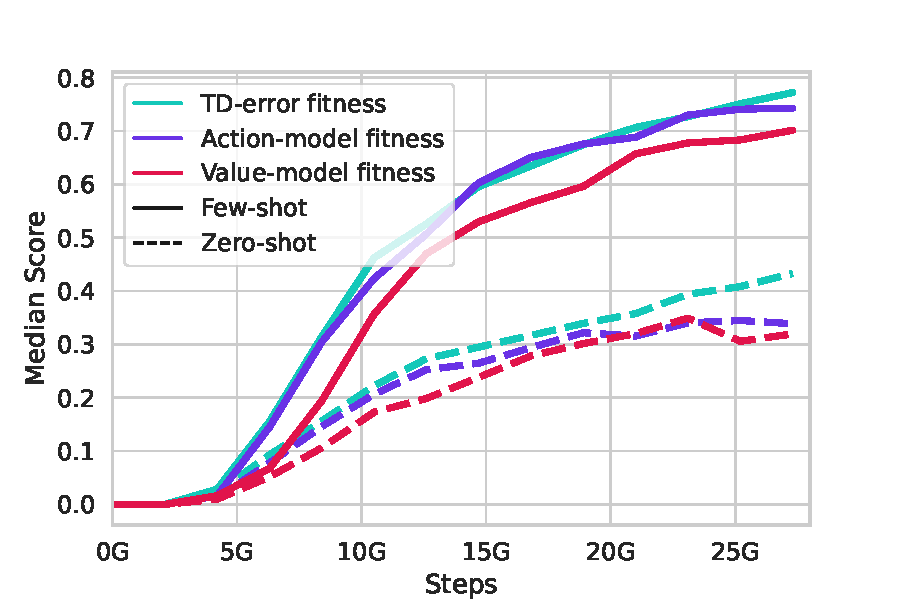
\includegraphics[width=0.6\linewidth]{figures/curriculum/autocurriculum_abl1.pdf}
    \caption{
         PLR fitness metric comparison for zero-shot generalisation ($k = 1$) and few-shot adaptation ($k = 13$). We compare the TD-error fitness used in our main agents against two approaches using the Muesli dynamics model. We see that action-model fitness matches TD-error fitness in few-shot performance, with weaker zero-shot performance.
    }
    \label{fig:autocurriculum_abl1}
\end{figure}

In Figure~\ref{fig:autocurriculum_abl1} we show training curves for TD-error fitness, value-model fitness, and action-model fitness. Table \ref{tab:fitness_functions} shows the experimental setup for these experiments. We see that both TD-error and action-model fitness metrics outperform the value-model fitness. We chose TD-error for our PLR training runs because it has better asymptotic performance in both the zero-shot and the few-shot setting, and because it was shown to perform well in previous work~\citep{jiang2021robustplr}.

\begin{table}[h!]
  \begin{center}
    \caption{Experimental setup for comparing different PLR fitness functions.}
    \begin{tabular}{c|c|c|c|c|c|c}
    \label{tab:fitness_functions}
      Model parameters & Memory & Task pool & Curriculum & Teacher & Steps & Fitness function \\
      \hline
      \multirow{3}{*}{23M TXL / 76M total} & 
      \multirow{3}{*}{1800} & 
      \multirow{3}{*}{25B} &
      \multirow{3}{*}{PLR} & 
      \multirow{3}{*}{None} & 
      \multirow{3}{*}{25B} & 
      TD error \\
       & & & & & & Value model \\ 
       & & & & & & Action model \\ 
    \end{tabular}
  \end{center}
\end{table}

\paragraph{Curriculum efficiency.}

\begin{figure}[htb]
    \centering
    \begin{subfigure}[b]{0.49\textwidth}
        \centering
        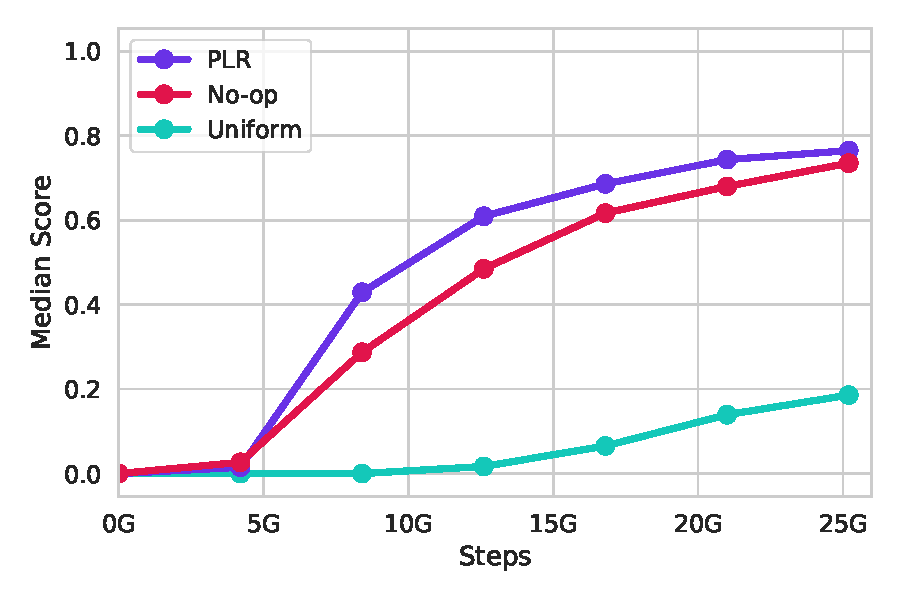
\includegraphics[width=\linewidth]{figures/curriculum/curricula_efficiency.pdf}
        \vskip -3pt \caption{}
    \end{subfigure}
    \begin{subfigure}[b]{0.49\textwidth}
        \centering
        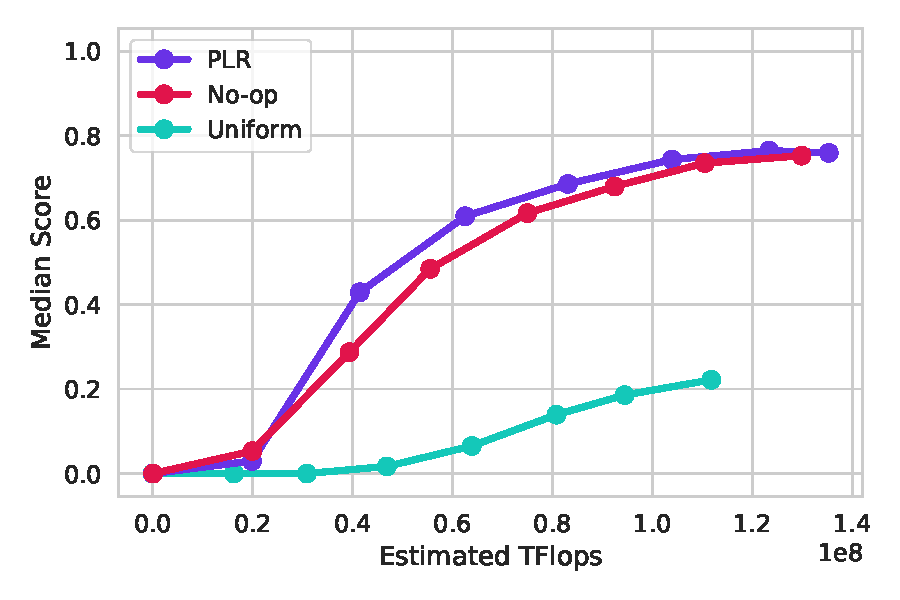
\includegraphics[width=\linewidth]{figures/curriculum/curricula_efficiency_flops.pdf}
        \vskip -3pt \caption{}
    \end{subfigure}
    \caption{
        \textbf{(a)} Sample efficiency in steps for different choices of curricula. Both No-op and PLR significantly improves sample efficiency over uniform sampling of tasks. Few-shot denotes $k=13$ score and zero-shot denotes $k=1$ score. 
        \textbf{(b)} Sample efficiency in FLOPs for different choices of curricula. No-op has an initial advantage over PLR, but PLR outperforms No-op later in training.
    }
\label{fig:curricula_efficiency}
\end{figure}

Next, we compare training sample efficiency for baseline uniform sampling and the different curriculum methods, in units of both learner steps and FLOPS. Figure~\ref{fig:curricula_efficiency} shows the median last-trial scores for few-shot ($k=13$) and zero-shot evaluation tasks as a function of learner steps. We see that both No-op filtering and PLR curricula strongly improve training sample efficiency over uniform sampling, with PLR being more efficient early in the training process. When we plot the same few-shot median performance as a function of FLOPS, we see that No-op has a slight early advantage, but PLR outperforms No-op later in training. The initial advantage for No-op may be because No-op expends more FLOPS (10 evaluations per task vs.~1 in PLR) for task evaluation, which finds higher quality training tasks at the start of training.

\paragraph{Emergent curricula.} In Figure~\ref{fig:emergent_curricula_extended} we show task metrics analysing the tasks selected by PLR and No-op filtering, expanding upon the results shown in Figure \ref{fig:emergent_curricula}.

\begin{figure}[h!]
    \centering
    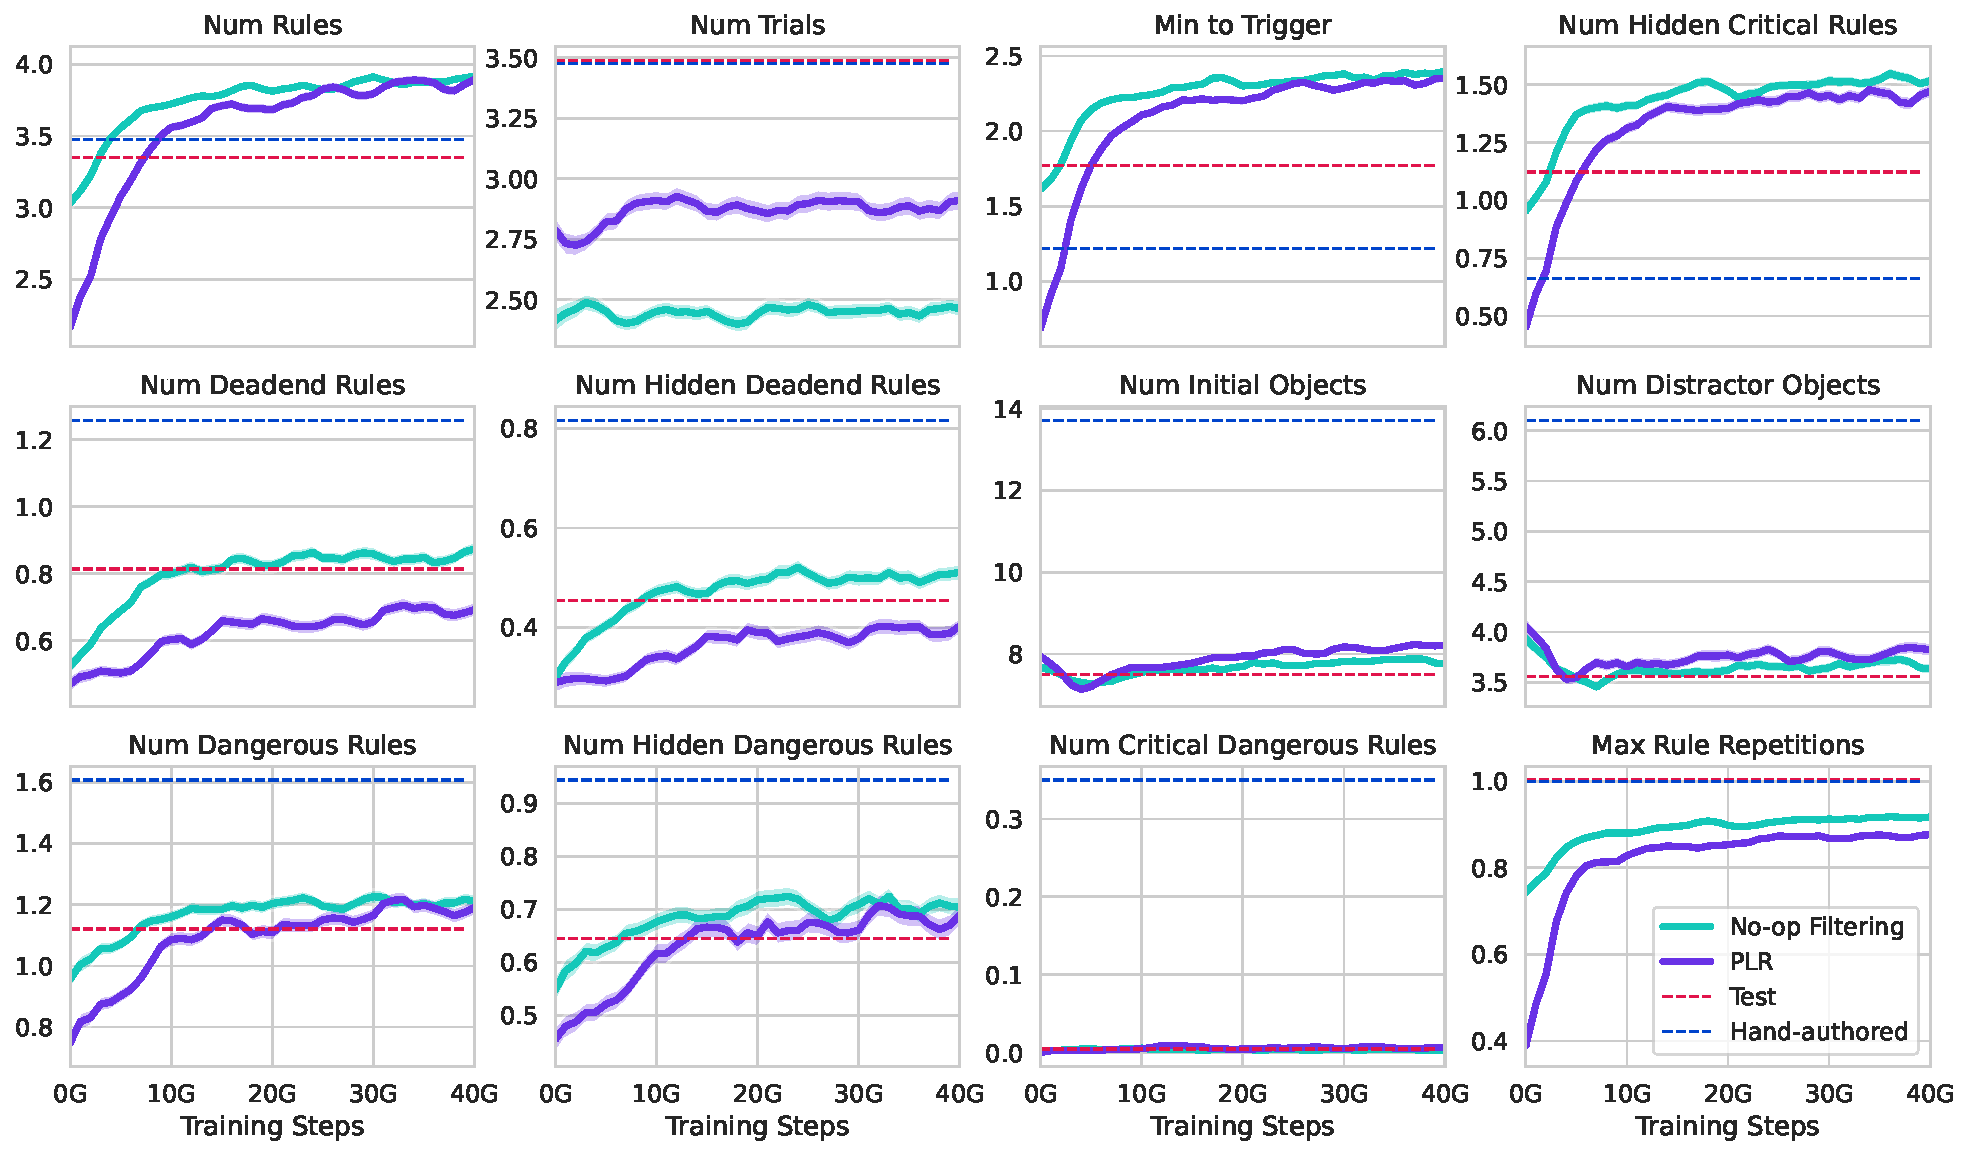
\includegraphics[width=0.99\linewidth]{figures/curriculum/emergent_curricula_extended.pdf}
    \caption{
        Emergent curricula for No-op filtering and PLR. Plots show the full set of task metrics for the dynamic training set, averaged over all tasks in the set, with standard error shaded. In all plots, a higher metric value corresponds to greater task difficulty. Horizontal lines show the same metric values averaged over the test (dashed) and hand-authored (dotted) evaluation task sets.}
    \label{fig:emergent_curricula_extended}
\end{figure}

\subsection{Distillation teacher for scaling experiments}
\label{app:scaling_distillation_teacher}
In all of our scaling experiments (Sections \ref{sec:scaling_results} and \ref{sec:results_task_scaling}), we distill the policy from an identical teacher snapshot to ensure our experiments are comparable. Training details for the teacher are detailed in Table \ref{tab:Teacher}. This teacher is used to kickstart our agents for their first 4B frames of training. 

\begin{table}[h!]
  \begin{center}
    \caption{Distillation teacher for scaling experiments.}
    \begin{tabular}{c|c|c|c|c|c}
    \label{tab:Teacher}
      Model parameters & Memory & Task pool & Curriculum & Teacher & Steps\\ % <--
      \hline
      23M TXL / 76M total & 1800 & 200M & No-op & None & 23B \\ % <--
    \end{tabular}
  \end{center}
\end{table}

\subsection{Scaling the network}
\label{app:network-scaling}
Table \ref{tab:model_scaling} shows the experimental setup for the model size scaling experiments in Section \ref{sec:scaling_results}. More details about the number of parameters for the various model sizes can be found in Table~\ref{tab:model_hparams}.

\begin{table}[t!]
  \begin{center}
    \caption{Experimental setup for model size scaling.}
    \begin{tabular}{c|c|c|c|c|c}
    \label{tab:model_scaling}
      Model parameters & Memory & Task pool & Curriculum  & Teacher & Steps \\ % <-- 
      \hline
      6M TXL / 41M total & \multirow{7}{*}{1800} & \multirow{7}{*}{25B} & \multirow{7}{*}{No-op} & \multirow{7}{*}{Table \ref{tab:Teacher}} & \multirow{7}{*}{75B}\\ % <--
      23M TXL / 76M total&&&&&\\ % <--
      42M TXL / 112M total&&&&&\\
      57M TXL / 141M total&&&&&\\
      75M TXL / 175M total&&&&&\\
      169M TXL / 353M total&&&&&\\
      265M TXL / 533M total&&&&&\\
    \end{tabular}
  \end{center}
\end{table}


Transformer-XL memory is a cached memory of previous attention layer inputs, concatenated to the keys and values during each forward pass. Inputs to intermediate layer are activations from the previous layer, which in themselves contain information about the past. Caching $M$ activations this way theoretically allows for an effective memory horizon of $M$ x $L$, where $L$ is the number of attention layers in the network.
Therefore, to avoid implicitly scaling effective Transformer-XL memory length, in our model size scaling experiments, we fix the number of layers in the Transformer, and scale parameters only by altering the Transformer embedding size ($d_\textrm{model}$), with the feed-forward size fixed at $4 d_\textrm{model}$, as is standard in Transformer architectures \citep{vaswani2017attention}.

\begin{table}[h!]
  \begin{center}
    \caption{Transformer hyperparameters for different model sizes.}
    \begin{tabular}{c|c|c|c|c|c|c}
    \label{tab:model_hparams}
      Model parameters & Embedding size & Blocks & Key size & Value size & Heads & FFW size\\
      \hline
      6M TXL / 41M total & 288 & 6 & 48 & 48 & 6 & 1152\\
      23M TXL / 76M total & 576 & 6 & 48 & 48 & 12 & 2304\\
      42M TXL / 112M total & 768 & 6 & 32 & 32 & 24 & 3072\\
      57M TXL / 141M total & 896 & 6 & 32 &32 & 28 & 3584\\
      75M TXL / 175M total & 1024 & 6 & 32 & 32 & 32 & 4096\\
      169M TXL / 353M total & 1536 & 6 & 48 & 48 & 32 & 6144\\
      265M TXL / 533M total & 1920 & 6 & 48 & 48 & 40 & 7680\\
    \end{tabular}
  \end{center}
\end{table}


\subsection{Scaling the memory length}
\label{app:memory-scaling}
Table \ref{tab:memory-scaling} shows the details of the experimental setup for the memory length scaling experiments in Section \ref{sec:scaling_results}. We show the effective memory timesteps for each experiment, computed as the number of cached network activations times the number of transformer blocks (6).

\begin{table}[h!]
  \begin{center}
    \caption{Experimental setup for scaling the memory length.}
    \begin{tabular}{c|c|c|c|c|c}
    \label{tab:memory-scaling}
      Model Parameters & Memory & Training task pool & Curriculum & Teacher & Training steps \\
      \hline
      \multirow{4}{*}{23M TXL / 76M total} & 600 & \multirow{4}{*}{200M} & \multirow{4}{*}{No-op} & \multirow{4}{*}{Table \ref{tab:Teacher}} & \multirow{4}{*}{25B}\\
      & 1800 &&&&\\
      & 3000 &&&&\\
      & 4200 &&&&\\
    \end{tabular}
  \end{center}
\end{table}

\subsection{Scaling the size of the task pool}
\label{app:task-scaling}
Table \ref{tab:task-scaling} shows the details of the experimental setup for scaling the size of the task pool in Section~\ref{sec:results_task_scaling}. 

\begin{table}[h!]
  \begin{center}
    \caption{Experimental setup for scaling the task pool size.}
    \begin{tabular}{c|c|c|c|c|c}
    \label{tab:task-scaling}
      Model parameters & Memory & Training task pool & Curriculum & Teacher & Training steps \\
      \hline
      \multirow{2}{*}{23M TXL / 76M total} & \multirow{4}{*}{1800} & 200M & \multirow{4}{*}{No-op} & \multirow{4}{*}{Table \ref{tab:Teacher}} & \multirow{4}{*}{25B}\\
      && 25B &&&\\
      \multirow{2}{*}{75M TXL / 175M total} &  & 200M & & & \\
      && 25B &&&\\
    \end{tabular}
  \end{center}
\end{table}

\subsection{Scaling the complexity of the task pool}
\label{app:task-complexity-scaling}
Table \ref{tab:task_complexity_scaling} shows the details of the experimental setup for scaling the complexity of the task pool in Appendix \ref{app:scaling_complexity}. In this experiment, the distillation teachers are different for the two agents we compare. Therefore we cannot disentangle the effects of distillation and task complexity. Nevertheless, the results remain indicative of the importance of task complexity. The teacher for the task distribution across multiple world topologies is trained as in Table \ref{tab:Teacher}. The teacher for the task distribution in a single room comes from a long lineage (> 6 generations) of distillation teachers starting with agents trained on XLand 1.0 \citep{xland}.

\begin{table}[h!]
  \begin{center}
    \caption{Experimental setup for scaling the complexity of the task distribution.}
    \begin{tabular}{c|c|c|c|c}
    \label{tab:task_complexity_scaling}
      Model parameters & Memory & Task pool & Curriculum  & Steps \\ % <-- 
      \hline
      6M TXL / 41M total & \multirow{5}{*}{1800} & \multirow{5}{*}{4k worlds $\times$ 50k games} & \multirow{5}{*}{No-op} & \multirow{5}{*}{23B}\\ % <--
      23M TXL / 76M total&&&&\\ % <--
      42M TXL / 112M total&&&&\\
      57M TXL / 141M total&&&&\\
      75M TXL / 175M total&&&&\\
      \hline
      6M TXL / 41M total &  \multirow{4}{*}{1800} & \multirow{4}{*}{1 world $\times$ 5k inits $\times$ 50k games} & \multirow{4}{*}{No-op}&\multirow{4}{*}{23B}\\ % <--
      23M TXL / 76M total&&&&\\ % <--
      42M TXL / 112M total&&&&\\
      57M TXL / 141M total&&&&\\
    \end{tabular}
  \end{center}
\end{table}


\subsection{Distillation enables scaling agents}
\label{app:distillation-exp}
Table \ref{tab:distillation-exp} shows the experimental setup for the distillation experiments in Section \ref{sec:results_kickstarting}.

\begin{table}[h!]
  \begin{center}
    \caption{Experimental setup for distillation experiments.}
    \begin{tabular}{c|c|c|c|c|c}
    \label{tab:distillation-exp}
      Model Parameters & Memory & Training task pool & Curriculum & Teacher & Steps\\
      \hline
      \multirow{2}{*}{TXL 23M TXL / 76M total} & \multirow{4}{*}{1800} & \multirow{4}{*}{See Sec~\ref{app:multi_agent_training}} & \multirow{4}{*}{PLR (\ref{tab:plr_hyperparameters})} &Table \ref{tab:multi-agent-teacher} & \multirow{4}{*}{22B}\\
      &&&&None&\\
      \multirow{2}{*}{TXL 265M TXL / 533M total}&&&& Table \ref{tab:multi-agent-teacher}&\\
      &&&&None&\\
    \end{tabular}
  \end{center}
\end{table}

\subsection{Training on more trials with skip memory}
\label{app:skip-memory-scaling}
Table \ref{tab:skip-memory-scaling} shows the details of the experimental setup for the memory scaling experiments in Section \ref{sec:results_few_to_many_shot}. This is the same setup as in Table \ref{tab:skip-memory-scaling}, except for the number of training steps and the variation of memory architecture and training trials discussed in the main text.

\begin{table}[h!]
  \begin{center}
    \caption{Experimental setup for experiments training on more trials with skip memory.}
    \begin{tabular}{c|c|c|c|c|c}
    \label{tab:skip-memory-scaling}
      Model Parameters & Memory & Training task pool & Curriculum & Teacher & Steps \\
      \hline
      \multirow{2}{*}{23M TXL / 76M total} & 1800 & \multirow{2}{*}{200M} & 
      \multirow{2}{*}{No-op} & 
      \multirow{2}{*}{Table \ref{tab:Teacher}} & \multirow{2}{*}{50B}\\
      & $1800 \times 4=7200$ &&&&\\
    \end{tabular}
  \end{center}
\end{table}
